\chapter{Resultados}

\section{Estratégia de validação}

Nesta seção, apresentam-se os resultados obtidos a partir das implementações computacionais desenvolvidas em GNU Octave. A validação foi organizada em duas etapas. Na primeira, considera-se um sistema linear periódico de dimensão \(2\times2\), com solução exata conhecida, com o objetivo de testar isoladamente a formulação de Fourier no tempo. Na segunda, considera-se a equação do calor bidimensional, discretizada no espaço por colocação espectral de Chebyshev e tratada no tempo por expansão de Fourier.

Em ambos os casos, utiliza-se uma solução exata fabricada. A forçante correspondente é construída por substituição direta na equação diferencial, de modo que a aproximação numérica possa ser comparada com uma solução conhecida. Esse procedimento fornece um ambiente controlado para avaliar o erro, o resíduo da equação e o número de condição dos sistemas lineares resolvidos.

Além das tabelas numéricas, os resultados são apresentados por meio de gráficos de erro, convergência, condicionamento e superfícies espaciais. As tabelas registram os valores quantitativos principais, enquanto os gráficos evidenciam tendências importantes, como a queda do erro com o refinamento, o crescimento do número de condição e a aproximação dos resíduos à precisão de máquina. Os códigos comentados utilizados nas simulações são apresentados no Apêndice, a fim de explicitar a ligação entre a formulação matemática e a implementação computacional.

\section{Validação temporal em um sistema \texorpdfstring{\(2\times2\)}{2x2}}

\subsection{Formulação do problema-teste}

O primeiro teste considera o sistema linear periódico
\[
U'(t)=AU(t)+b(t),
\]
obtido a partir da equação escalar de segunda ordem
\[
x''(t)+x'(t)+x(t)=f(t),
\qquad t\in\mathbb{R},
\]
com período \(T=2\pi\). Escolhe-se como solução exata
\[
x_{\mathrm{ex}}(t)=\sin t+\cos(2t).
\]
Derivando, obtém-se
\[
x'_{\mathrm{ex}}(t)=\cos t-2\sin(2t),
\qquad
x''_{\mathrm{ex}}(t)=-\sin t-4\cos(2t),
\]
e, portanto,
\[
f(t)=x''_{\mathrm{ex}}(t)+x'_{\mathrm{ex}}(t)+x_{\mathrm{ex}}(t)
=-3\cos(2t)+\cos t-2\sin(2t).
\]

Para escrever o problema como sistema de primeira ordem, introduz-se
\[
u=x,
\qquad v=x'.
\]
Assim,
\[
u'=v,
\qquad
v'=-u-v+f(t),
\]
o que conduz a
\[
\frac{d}{dt}
\begin{bmatrix}
u\\ v
\end{bmatrix}
=
\begin{bmatrix}
0 & 1\\
-1 & -1
\end{bmatrix}
\begin{bmatrix}
u\\ v
\end{bmatrix}
+
\begin{bmatrix}
0\\ f(t)
\end{bmatrix}.
\]
Esse exemplo é adequado para validar a etapa temporal do método, pois a solução é composta apenas por poucos harmônicos. Como aparece o termo \(\cos(2t)\), espera-se que a aproximação por Fourier recupere a solução com alta precisão assim que o modo \(k=2\) for incluído.

\subsection{Resultados obtidos}

A Tabela~\ref{tab:sistema2x2_modos} apresenta os resultados obtidos para diferentes valores de \(K\). Para cada valor de \(K\), utiliza-se \(N_t=2K+1\) pontos temporais no período. A tabela registra o erro máximo na primeira componente da solução e o resíduo máximo do sistema. O número de condição das matrizes modais é calculado nos códigos como diagnóstico auxiliar de estabilidade numérica.

\begin{table}[h!]
\centering
\caption{Validação do algoritmo temporal no sistema \(2\times2\) para diferentes valores de \(K\).}
\label{tab:sistema2x2_modos}
\begin{tabular}{cccc}
\toprule
\(K\) & \(N_t\) & Erro máximo & Resíduo máximo \\
\midrule
1  & 3   & \(4.2832\times 10^{0}\)  & \(6.5415\times 10^{0}\) \\
2  & 5   & \(1.3323\times 10^{-15}\) & \(2.6645\times 10^{-15}\) \\
4  & 9   & \(1.7764\times 10^{-15}\) & \(4.4409\times 10^{-15}\) \\
8  & 17  & \(1.5543\times 10^{-15}\) & \(3.5527\times 10^{-15}\) \\
16 & 33  & \(1.1102\times 10^{-15}\) & \(5.7732\times 10^{-15}\) \\
32 & 65  & \(6.6613\times 10^{-16}\) & \(5.3291\times 10^{-15}\) \\
64 & 129 & \(1.1102\times 10^{-15}\) & \(4.4409\times 10^{-15}\) \\
\bottomrule
\end{tabular}
\end{table}

Para \(K=1\), o erro ainda é significativo, indicando que o número de modos de Fourier é insuficiente para representar a solução. Isso é esperado, pois a solução exata contém o modo de frequência \(2\), associado ao termo \(\cos(2t)\). A partir de \(K=2\), esse modo passa a estar presente na base temporal truncada, e o erro decai abruptamente para a ordem de \(10^{-15}\), isto é, para valores compatíveis com a precisão de máquina.

Esse comportamento evidencia a natureza espectral do método. Uma vez incluídos os modos relevantes da solução exata, a aproximação torna-se essencialmente exata, e os erros restantes passam a ser dominados por efeitos de arredondamento numérico. Esse resultado está de acordo com a teoria de decaimento dos coeficientes espectrais discutida na Seção~\ref{sec:decaimento-aliasing-gibbs}: neste caso particular, a série de Fourier da solução possui apenas um número finito de modos. A Figura~\ref{fig:convergencia_sistema2x2} mostra essa queda abrupta do erro com o aumento de \(K\).

\begin{figure}[h!]
\centering
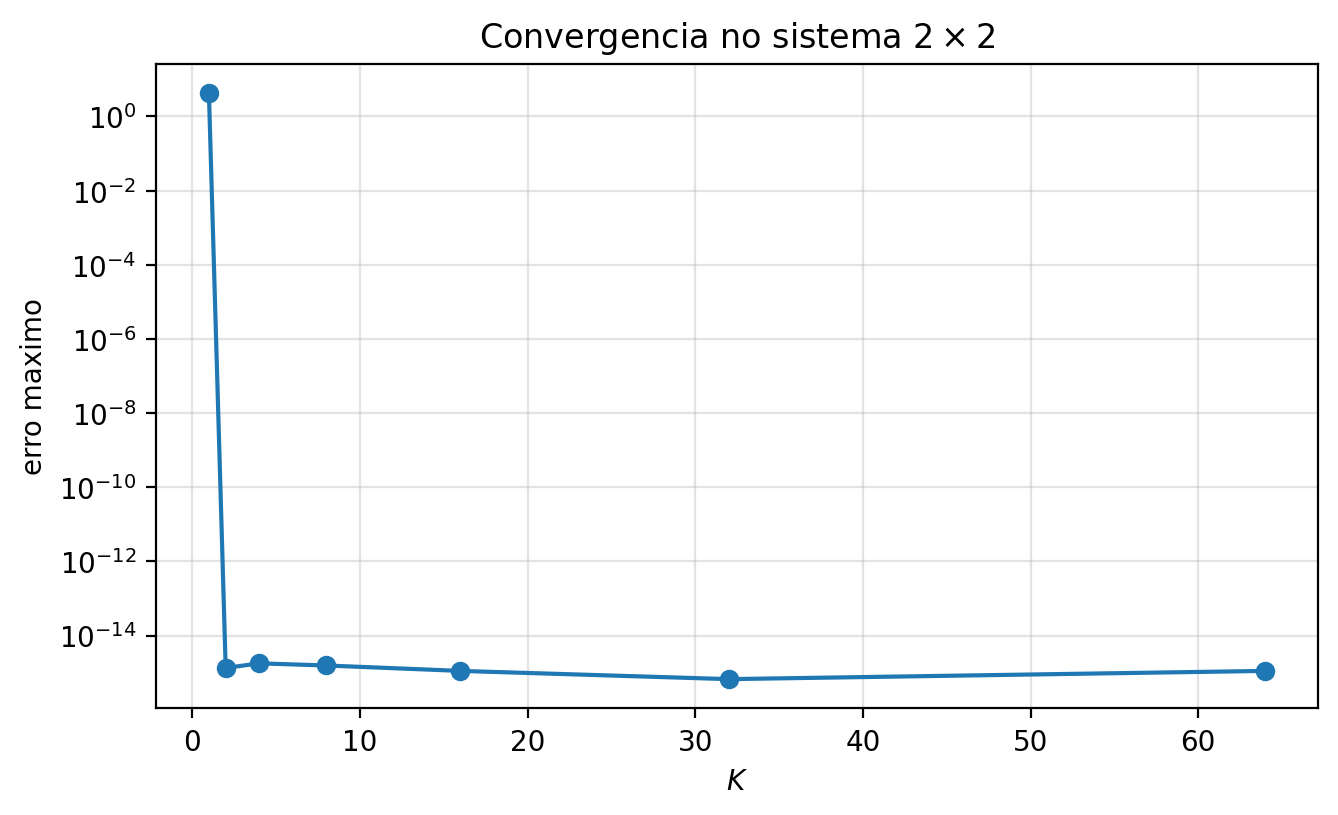
\includegraphics[width=0.78\textwidth]{figuras/grafico_convergencia_sistema2x2.png}
\caption{Convergência do erro máximo no sistema \(2\times2\) em função do número de modos de Fourier.}
\label{fig:convergencia_sistema2x2}
\end{figure}

A Figura~\ref{fig:erro_sistema2x2_k8} apresenta o erro ao longo do tempo para \(K=8\). Observa-se que o erro permanece da ordem de \(10^{-15}\), confirmando que a solução reconstruída coincide com a solução exata até erros de arredondamento.

\begin{figure}[h!]
\centering
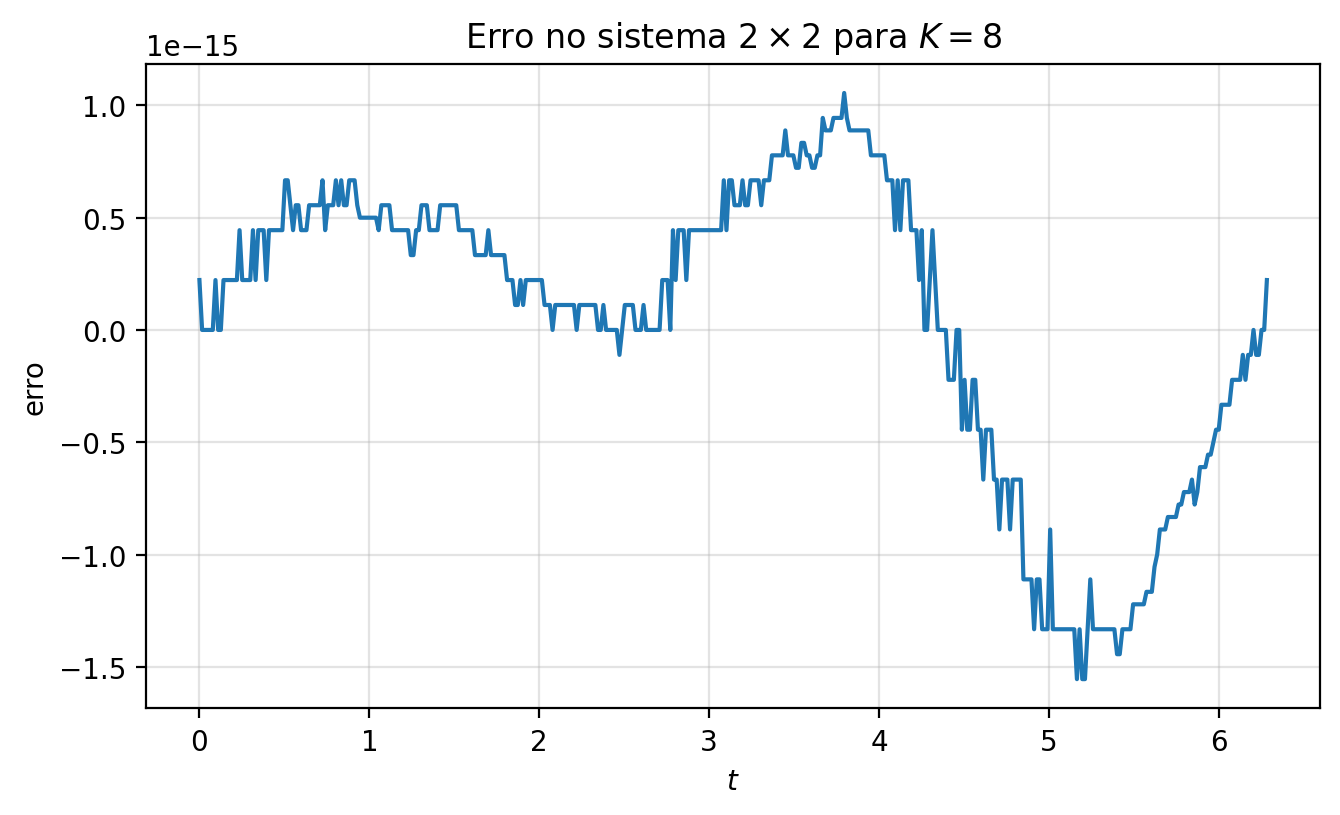
\includegraphics[width=0.78\textwidth]{figuras/grafico_erro_sistema2x2_K8.png}
\caption{Erro na primeira componente do sistema \(2\times2\) para \(K=8\).}
\label{fig:erro_sistema2x2_k8}
\end{figure}

Além do erro, calcula-se o resíduo
\[
R_K(t)=X_K'(t)-AX_K(t)-b(t),
\]
que mede o quanto a solução aproximada satisfaz o sistema diferencial. A Figura~\ref{fig:residuo_sistema2x2} mostra que, a partir de \(K=2\), o resíduo também permanece próximo da precisão de máquina. Esse resultado é importante porque, em problemas sem solução exata conhecida, o resíduo passa a ser um dos principais critérios de validação.

\begin{figure}[h!]
\centering
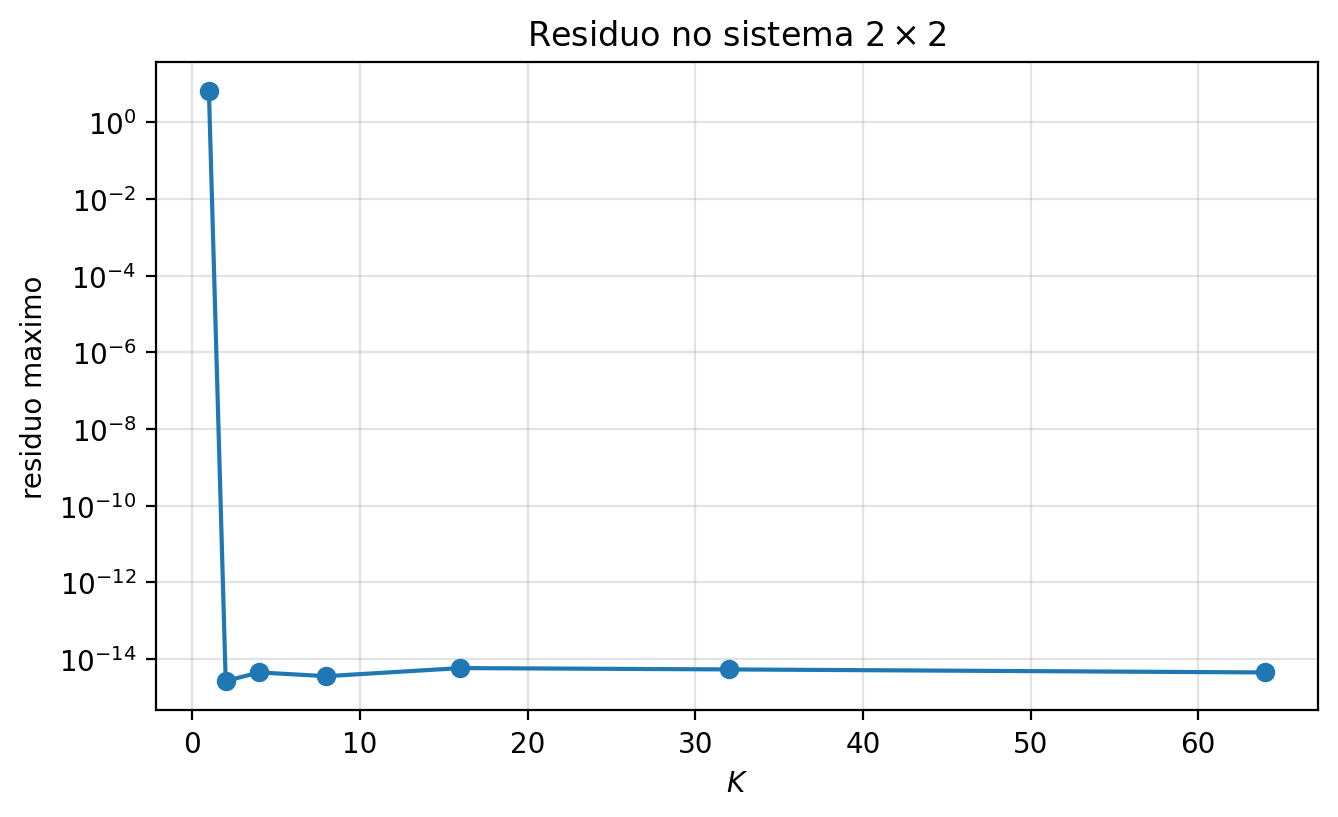
\includegraphics[width=0.78\textwidth]{figuras/grafico_residuo_sistema2x2.png}
\caption{Resíduo máximo do sistema \(2\times2\) em função de \(K\).}
\label{fig:residuo_sistema2x2}
\end{figure}

\section{Conexão entre os dois códigos}
\label{sec:conexao-codigos}

A passagem do primeiro problema de validação para o segundo problema não representa uma mudança de método, mas uma ampliação natural da mesma ideia algorítmica. No primeiro teste, parte-se diretamente de um sistema linear finito-dimensional da forma
\[
U'(t)=AU(t)+b(t),
\]
no qual a matriz \(A\) é pequena e dada explicitamente. Esse problema permite validar, de maneira isolada, a etapa temporal do método: a decomposição em modos de Fourier, o cálculo dos coeficientes da forçante por FFT, a resolução dos sistemas lineares modo a modo e a reconstrução da solução periódica.

No segundo código, o ponto de partida é a equação do calor bidimensional periódica no tempo,
\[
u_t=\Delta u+f,
\]
definida em um domínio espacial limitado. Nesse caso, antes de aplicar Fourier na variável temporal, é necessário discretizar o operador espacial \(\Delta\). Essa discretização é feita por colocação espectral de Chebyshev nas variáveis espaciais. Como consequência, a EDP é transformada em um sistema semidiscreto de equações diferenciais ordinárias no tempo,
\[
U'(t)=AU(t)+b(t),
\]
em que \(U(t)\) contém os valores aproximados da solução nos pontos internos da malha de Chebyshev, \(A\) representa o Laplaciano discreto e \(b(t)\) representa a forçante avaliada nesses mesmos pontos.

Dessa forma, depois da discretização espacial, reaparece exatamente a mesma estrutura algébrica estudada no sistema finito-dimensional. A diferença é que, no primeiro código, a matriz \(A\) é uma matriz \(2\times2\) escolhida a partir de uma equação diferencial ordinária de segunda ordem; no segundo código, \(A\) é uma matriz de dimensão maior, construída a partir das matrizes de diferenciação de Chebyshev e da soma de Kronecker que representa o Laplaciano bidimensional.

Assim, o elo central entre os dois códigos pode ser resumido por
\[
\text{EDP do calor}
\quad \xrightarrow{\text{Chebyshev no espaço}} \quad
U'(t)=AU(t)+b(t)
\quad \xrightarrow{\text{Fourier no tempo}} \quad
(ik\omega I-A)\widehat{U}_k=\widehat{b}_k.
\]
Portanto, o primeiro código valida o núcleo temporal do algoritmo, enquanto o segundo mostra como esse núcleo é incorporado a uma formulação Fourier--Chebyshev para uma equação diferencial parcial.

A Figura~\ref{fig:conexao-codigos} resume essa relação entre as duas implementações.

\begin{figure}[h!]
\centering
\begin{tikzpicture}[
    node distance=0.78cm,
    >=Latex,
    bloco/.style={
        rectangle,
        rounded corners,
        draw,
        align=center,
        minimum width=7.8cm,
        minimum height=0.82cm,
        font=\small
    },
    seta/.style={->, thick}
]

\node[bloco] (c1) {Código 1: sistema finito-dimensional\\
\(U'(t)=AU(t)+b(t)\)};

\node[bloco, below=of c1] (four1) {Validação da etapa temporal\\
Fourier no tempo, FFT para \(\widehat{b}_k\) e resolução de\\
\((ik\omega I-A)\widehat{U}_k=\widehat{b}_k\)};

\node[bloco, below=of four1] (edp) {Código 2: equação do calor bidimensional periódica\\
\(u_t=\Delta u+f\)};

\node[bloco, below=of edp] (cheb) {Discretização espacial por Chebyshev\\
colocação espectral nos pontos internos};

\node[bloco, below=of cheb] (semi) {Sistema semidiscreto resultante\\
\(U'(t)=AU(t)+b(t)\)};

\node[bloco, below=of semi] (four2) {Aplicação da mesma etapa temporal\\
Fourier no tempo, FFT e resolução modal};

\draw[seta] (c1) -- (four1);
\draw[seta] (four1) -- (edp);
\draw[seta] (edp) -- (cheb);
\draw[seta] (cheb) -- (semi);
\draw[seta] (semi) -- (four2);

\end{tikzpicture}
\caption{Conexão entre o problema finito-dimensional e a formulação Fourier--Chebyshev para a equação do calor.}
\label{fig:conexao-codigos}
\end{figure}

\section{Equação do calor bidimensional periódica}

\subsection{Formulação Fourier--Chebyshev}

Como segundo problema de teste, considera-se a equação do calor bidimensional
\[
u_t(x,y,t)=\Delta u(x,y,t)+f(x,y,t),
\qquad (x,y)\in(-1,1)\times(-1,1),
\]
com condições de contorno homogêneas de Dirichlet na fronteira e periodicidade temporal de período \(T=2\pi\):
\[
u(x,y,t+2\pi)=u(x,y,t).
\]
Esse problema representa a etapa em que a formulação temporal de Fourier, previamente validada em um sistema finito-dimensional, passa a ser combinada com uma discretização espectral espacial. A escolha de uma solução fabricada suave é deliberada: nesse regime, os coeficientes espectrais tendem a decair rapidamente, favorecendo o comportamento de convergência espectral descrito na Seção~\ref{sec:decaimento-aliasing-gibbs}.

Para discretizar o espaço, utilizam-se pontos de Chebyshev--Gauss--Lobatto. Se \(N_M\) é o parâmetro de discretização espacial, consideram-se os pontos
\[
x_j=\cos\left(\frac{j\pi}{N_M}\right),
\qquad j=0,1,\dots,N_M.
\]
Como a condição de contorno é homogênea de Dirichlet, os valores da solução na fronteira já são conhecidos e iguais a zero. Portanto, as incógnitas numéricas são tomadas apenas nos pontos internos.

A matriz de diferenciação de Chebyshev \(D\) aproxima a derivada primeira nos pontos de colocação, e \(D^2\) aproxima a derivada segunda. Após remover as linhas e colunas associadas aos pontos de fronteira, constrói-se o Laplaciano discreto bidimensional por soma de Kronecker:
\[
A=I\otimes D^2+D^2\otimes I.
\]
Assim, a equação do calor é transformada no sistema semidiscreto
\[
U'(t)=AU(t)+b(t),
\]
em que \(U(t)\) contém os valores aproximados de \(u(x_i,y_j,t)\) nos pontos internos, e \(b(t)\) contém os valores da forçante nesses mesmos pontos.

Como o problema é periódico no tempo, introduz-se
\[
\omega=\frac{2\pi}{T}
\]
e procuram-se aproximações truncadas da forma
\[
U_K(t)=\sum_{k=-K}^{K}\widehat{U}_k e^{ik\omega t},
\qquad
b_K(t)=\sum_{k=-K}^{K}\widehat{b}_k e^{ik\omega t}.
\]
Substituindo no sistema semidiscreto, obtém-se, para cada modo temporal,
\[
(ik\omega I-A)\widehat{U}_k=\widehat{b}_k,
\qquad k=-K,\dots,K.
\]
Portanto, a EDP periódica é reduzida a uma família finita de sistemas lineares independentes, um para cada frequência temporal considerada.

\subsection{Validação por solução fabricada}

Para validar o método, escolhe-se a solução exata
\[
u_{\mathrm{ex}}(x,y,t)
=
-\cos(t)\sin\bigl(\pi\cos(\pi x)\bigr)
\sin\bigl(\pi\cos(\pi y)\bigr).
\]
Essa função é \(2\pi\)-periódica no tempo, pois depende de \(\cos(t)\). Além disso, satisfaz as condições homogêneas de Dirichlet na fronteira. De fato, se \(x=\pm1\), então
\[
\cos(\pi x)=\cos(\pm\pi)=-1
\]
e, portanto,
\[
\sin(\pi\cos(\pi x))=\sin(-\pi)=0.
\]
Logo, \(u_{\mathrm{ex}}(\pm1,y,t)=0\). O mesmo raciocínio vale para \(y=\pm1\).

A forçante é obtida por substituição direta na equação do calor:
\[
f=u_t-\Delta u.
\]
Escrevendo
\[
g(x)=\sin\bigl(\pi\cos(\pi x)\bigr),
\qquad
h(y)=\sin\bigl(\pi\cos(\pi y)\bigr),
\]
temos
\[
u_{\mathrm{ex}}(x,y,t)=-\cos(t)g(x)h(y),
\]
logo
\[
u_t(x,y,t)=\sin(t)g(x)h(y).
\]
As derivadas espaciais \(u_{xx}\) e \(u_{yy}\) são calculadas analiticamente e implementadas na rotina da forçante. Esse procedimento, conhecido como solução fabricada, permite validar o método em um caso no qual a solução exata é conhecida previamente.

\subsection{Resultados obtidos}

Nos experimentos desta etapa, manteve-se fixo \(K=8\) para a aproximação de Fourier no tempo e variou-se o número de pontos de Chebyshev na discretização espacial. Essa escolha permite observar de maneira mais direta o efeito do refinamento espacial na precisão do método, uma vez que a dependência temporal da solução exata envolve essencialmente o fator \(-\cos(t)\).

Os resultados obtidos estão resumidos na Tabela~\ref{tab:calor2d}. Nesta versão, o erro principal é o erro máximo absoluto
\[
erro_{\max}=\max |U_{\mathrm{aprox}}-U_{\mathrm{ex}}|,
\]
calculado sobre todos os pontos internos e todos os tempos da malha de Fourier. Essa métrica é mais direta para avaliar a maior discrepância ponto a ponto entre a solução aproximada e a solução fabricada. A soma total dos erros em norma \(1\), usada em versões preliminares do experimento, foi mantida apenas como diagnóstico secundário, pois cresce com o número de pontos da malha e não mede diretamente o maior erro pontual.

\begin{table}[h!]
\centering
\caption{Desempenho numérico da formulação Fourier--Chebyshev para a equação do calor bidimensional periódica, com \(K=8\).}
\label{tab:calor2d}
\begin{tabular}{cccc}
\toprule
\(N_{\text{Cheb}}\) & Condição máxima & Erro máximo absoluto & Erro \(L^1\) total \\
\midrule
8  & \(1.8242\times 10^{2}\) & \(2.7111\times 10^{0}\)  & \(3.8747\times 10^{2}\) \\
16 & \(2.6766\times 10^{3}\) & \(2.0527\times 10^{-2}\) & \(8.4757\times 10^{0}\) \\
32 & \(4.1914\times 10^{4}\) & \(1.1682\times 10^{-6}\) & \(2.0972\times 10^{-3}\) \\
60 & \(5.0538\times 10^{5}\) & \(1.75\times 10^{-14}\) & \(\mathcal{O}(10^{-10})\) \\
80 & \(1.60\times 10^{6}\)  & \(2.53\times 10^{-14}\) & \(\mathcal{O}(10^{-10})\) \\
\bottomrule
\end{tabular}
\end{table}

A distinção entre as duas últimas colunas é importante. Os valores anteriormente reportados como erro principal correspondiam, na prática, ao diagnóstico acumulado em norma \(1\). Após a correção, o erro máximo absoluto mostra diretamente a maior diferença ponto a ponto entre a solução numérica e a solução fabricada. Esse ajuste torna a interpretação dos resultados mais clara e compatível com a métrica usual de erro em norma infinito.

Os resíduos máximos permaneceram próximos da precisão de máquina, com valores da ordem de \(10^{-13}\) a \(10^{-11}\), indicando que os sistemas lineares modais foram resolvidos de modo consistente. Para os maiores valores de \(N_{\text{Cheb}}\), as pequenas variações numéricas são dominadas por arredondamento e pelo aumento do condicionamento.

A Figura~\ref{fig:erro_calor2d_ncheb} mostra a queda do erro máximo com o refinamento espacial. Observa-se que o erro passa de valores da ordem de \(10^0\), para \(N_{\text{Cheb}}=8\), para valores próximos da precisão de máquina quando \(N_{\text{Cheb}}\) é aumentado. Essa redução acentuada é compatível com o comportamento esperado de métodos espectrais quando aplicados a soluções suficientemente regulares. A pequena perda relativa de estabilidade observada no regime de erro de máquina é coerente com o crescimento do condicionamento das matrizes espectrais.

\begin{figure}[h!]
\centering
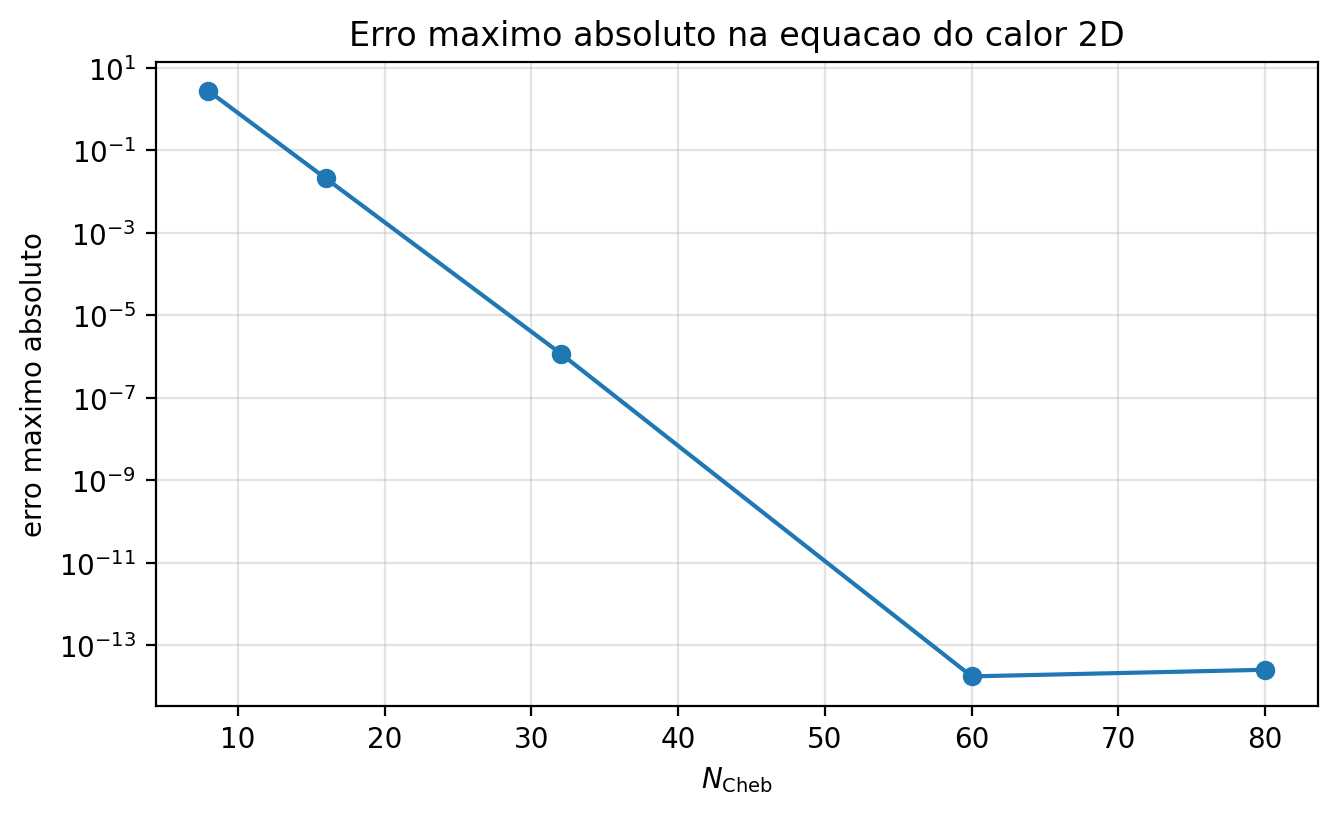
\includegraphics[width=0.78\textwidth]{figuras/grafico_erro_calor2d.png}
\caption{Erro máximo absoluto em função do número de pontos de Chebyshev para a equação do calor bidimensional.}
\label{fig:erro_calor2d_ncheb}
\end{figure}

A principal razão para essa queda rápida está na suavidade da solução exata e na adequação dos pontos de Chebyshev para representar funções regulares em intervalos limitados. Como a solução fabricada contém fatores espaciais suaves da forma
\[
\sin\bigl(\pi\cos(\pi x)\bigr)
\quad \text{e} \quad
\sin\bigl(\pi\cos(\pi y)\bigr),
\]
o aumento de \(N_{\text{Cheb}}\) permite capturar com maior precisão a estrutura espacial da solução.

Por outro lado, a Figura~\ref{fig:cond_calor2d_ncheb} mostra que o número de condição dos sistemas modais cresce significativamente com o refinamento espacial. Esse comportamento é típico de métodos espectrais baseados em matrizes de diferenciação, pois as matrizes associadas a operadores diferenciais tornam-se progressivamente mais mal condicionadas à medida que o número de pontos aumenta.

\begin{figure}[h!]
\centering
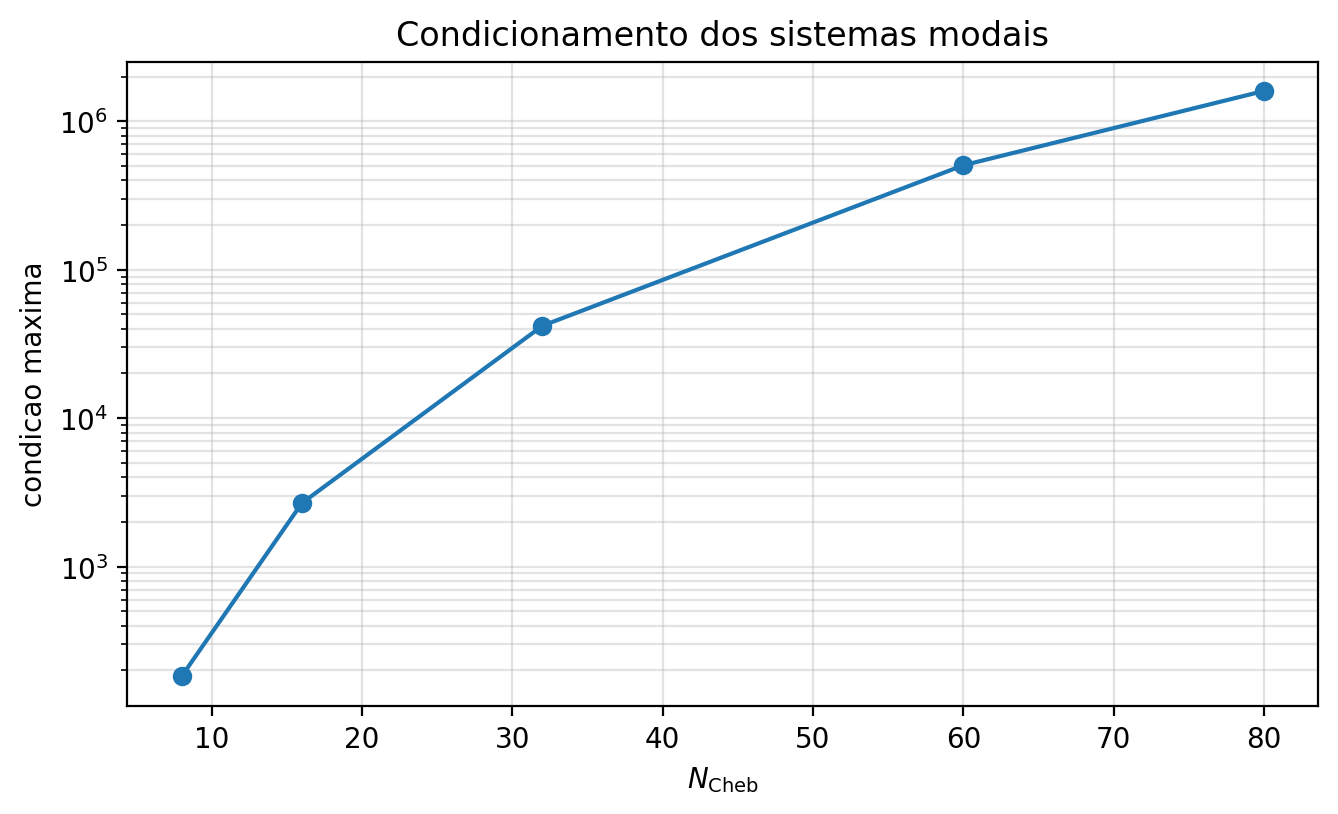
\includegraphics[width=0.78\textwidth]{figuras/grafico_condicao_calor2d.png}
\caption{Número de condição máximo dos sistemas modais em função de \(N_{\text{Cheb}}\).}
\label{fig:cond_calor2d_ncheb}
\end{figure}

A análise conjunta do erro e do condicionamento é apresentada na Figura~\ref{fig:erro_cond_calor2d}. Observa-se um compromisso entre precisão e estabilidade numérica: o aumento de \(N_{\text{Cheb}}\) melhora a representação espacial da solução, mas também torna os sistemas lineares mais sensíveis a erros de arredondamento.

\begin{figure}[h!]
\centering
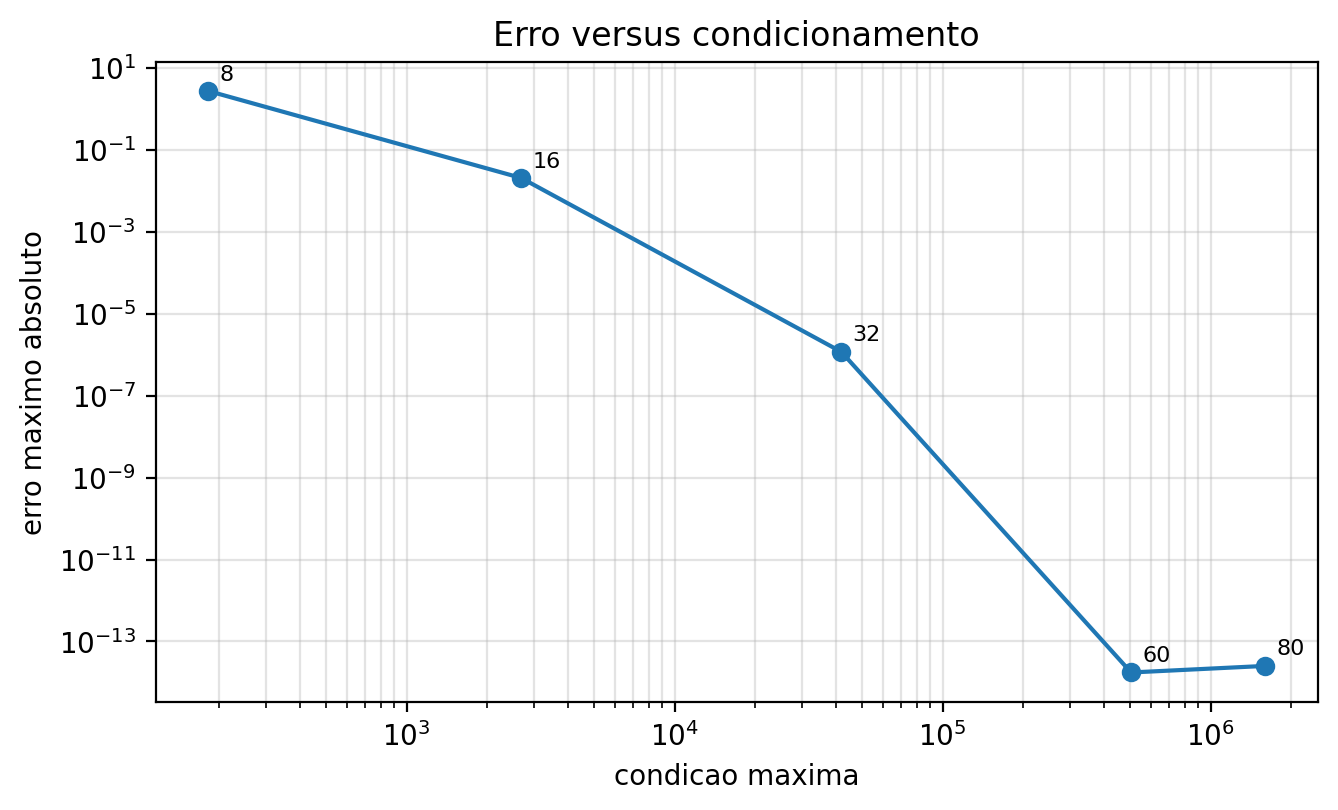
\includegraphics[width=0.78\textwidth]{figuras/grafico_erro_vs_condicao_calor2d.png}
\caption{Relação entre erro máximo absoluto e número de condição máximo na formulação Fourier--Chebyshev.}
\label{fig:erro_cond_calor2d}
\end{figure}

Apesar do crescimento do condicionamento, os resíduos permanecem próximos da precisão de máquina, como mostra a Figura~\ref{fig:residuo_calor2d}. Isso indica que os sistemas lineares modais foram resolvidos de maneira consistente e que a solução reconstruída satisfaz o sistema semidiscreto com alta acurácia.

\begin{figure}[h!]
\centering
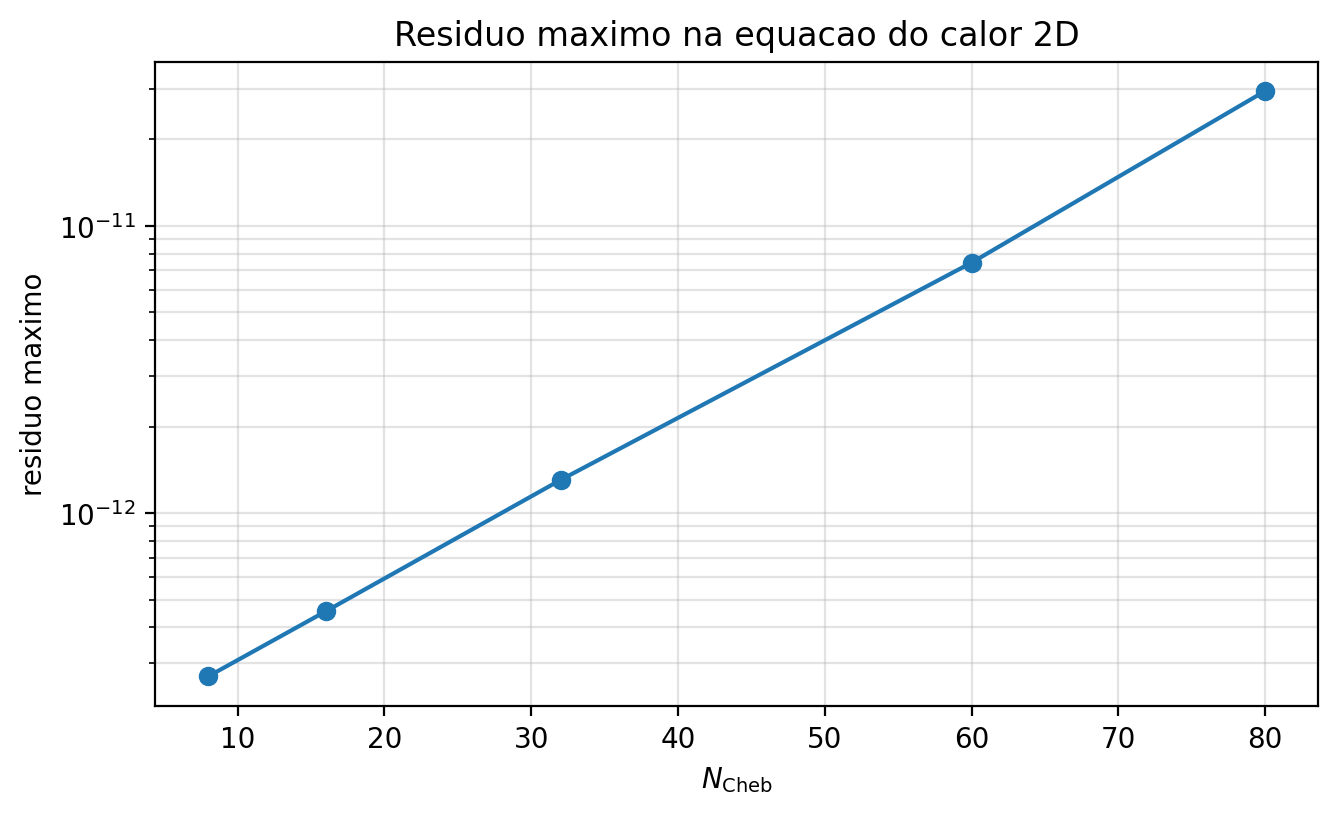
\includegraphics[width=0.78\textwidth]{figuras/grafico_residuo_calor2d.png}
\caption{Resíduo máximo da equação do calor bidimensional em função de \(N_{\text{Cheb}}\).}
\label{fig:residuo_calor2d}
\end{figure}

As superfícies da solução aproximada e do erro espacial fornecem uma visualização qualitativa do refinamento. As Figuras~\ref{fig:solucao_calor_n8}, \ref{fig:solucao_calor_n16} e \ref{fig:solucao_calor_n32} mostram a solução aproximada no instante \(t=0\) para diferentes valores de \(N_{\text{Cheb}}\). Com o aumento da resolução espacial, a superfície passa a representar melhor a estrutura oscilatória da solução fabricada.

\begin{figure}[h!]
\centering
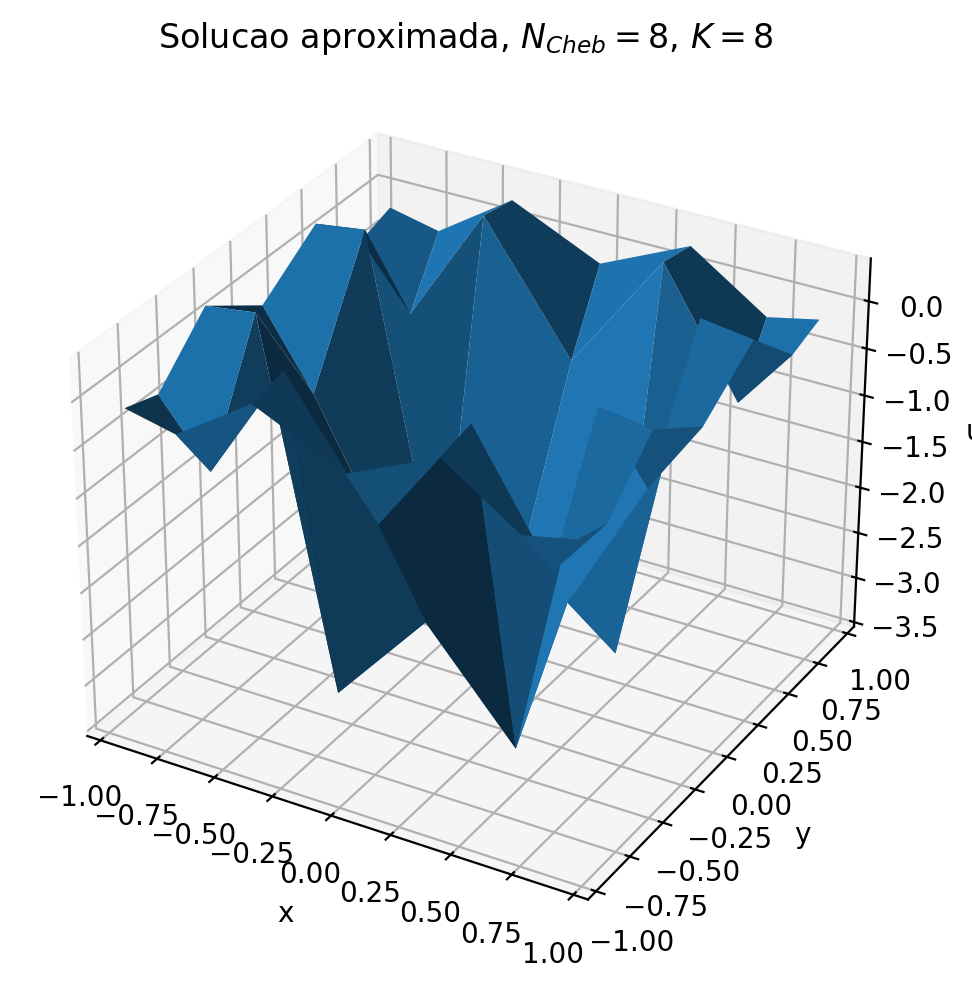
\includegraphics[width=0.72\textwidth]{figuras/superficie_solucao_calor2d_N8_K8.png}
\caption{Solução aproximada no instante \(t=0\), com \(N_{\text{Cheb}}=8\) e \(K=8\).}
\label{fig:solucao_calor_n8}
\end{figure}

\begin{figure}[h!]
\centering
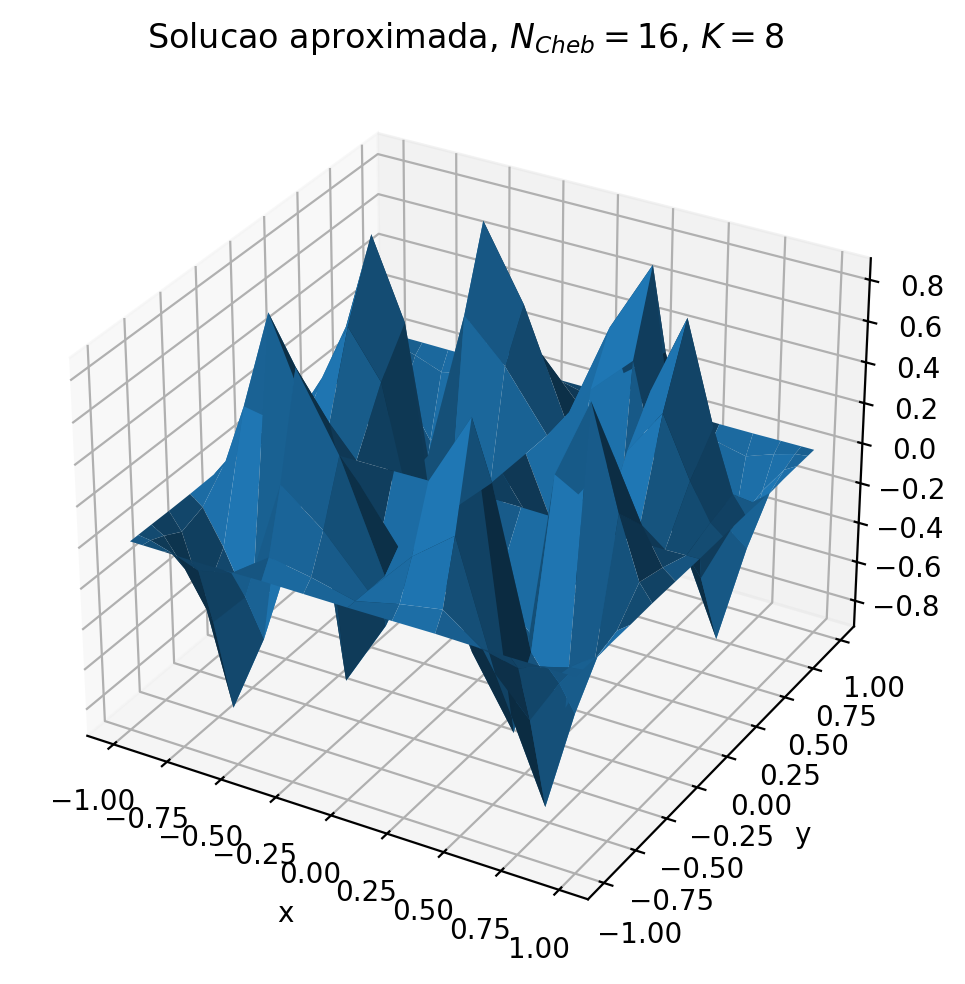
\includegraphics[width=0.72\textwidth]{figuras/superficie_solucao_calor2d_N16_K8.png}
\caption{Solução aproximada no instante \(t=0\), com \(N_{\text{Cheb}}=16\) e \(K=8\).}
\label{fig:solucao_calor_n16}
\end{figure}

\begin{figure}[h!]
\centering
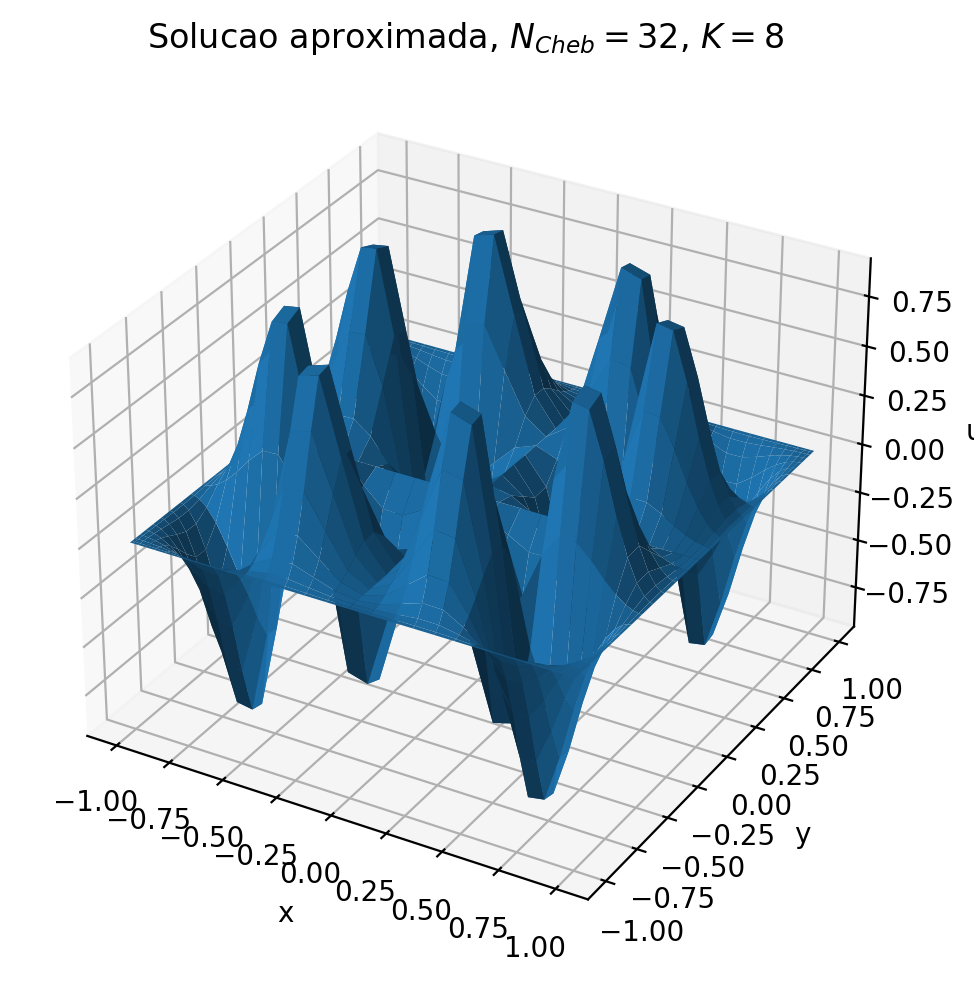
\includegraphics[width=0.72\textwidth]{figuras/superficie_solucao_calor2d_N32_K8.png}
\caption{Solução aproximada no instante \(t=0\), com \(N_{\text{Cheb}}=32\) e \(K=8\).}
\label{fig:solucao_calor_n32}
\end{figure}

As Figuras~\ref{fig:erro_espacial_n8}, \ref{fig:erro_espacial_n16} e \ref{fig:erro_espacial_n32} mostram o erro espacial correspondente. Para \(N_{\text{Cheb}}=8\), o erro ainda é elevado. Para \(N_{\text{Cheb}}=16\), observa-se redução significativa. Para \(N_{\text{Cheb}}=32\), o erro atinge valores muito pequenos, da ordem de \(10^{-6}\) na malha considerada, confirmando a melhora da aproximação com o refinamento espacial.

\begin{figure}[h!]
\centering
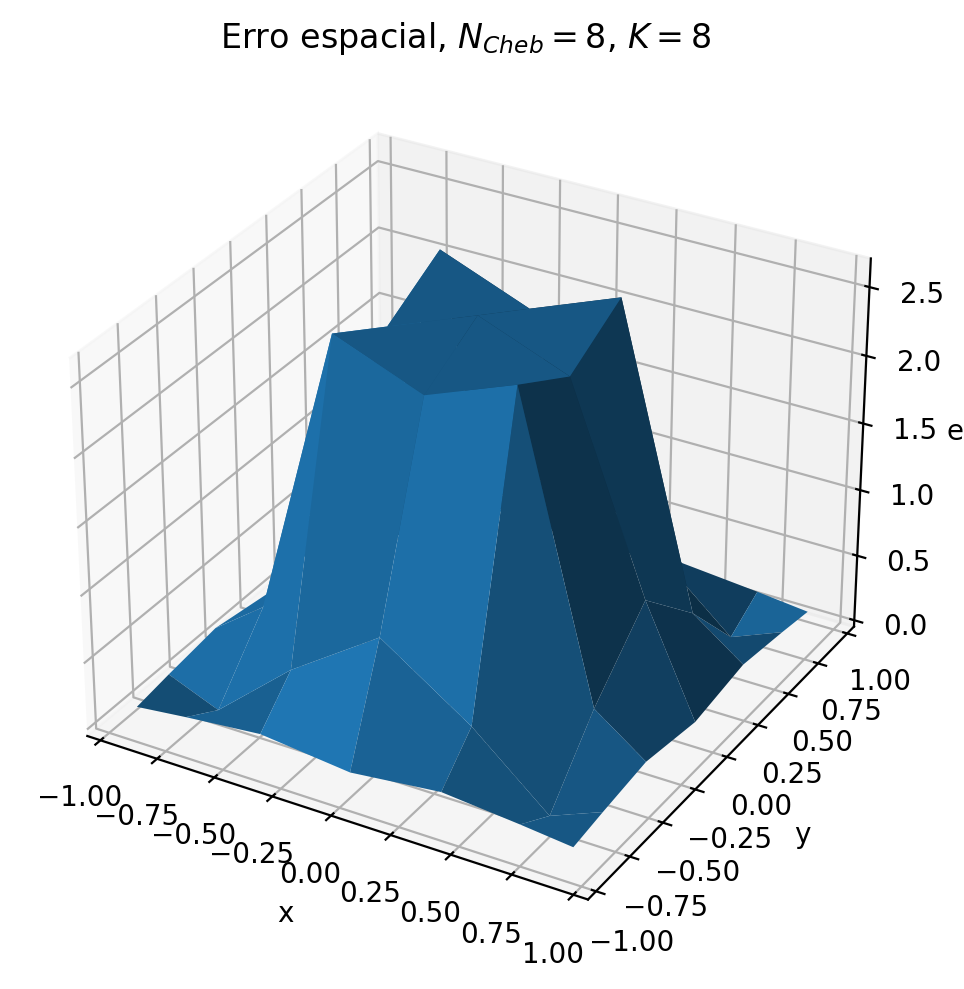
\includegraphics[width=0.72\textwidth]{figuras/superficie_erro_calor2d_N8_K8.png}
\caption{Erro espacial no instante \(t=0\), com \(N_{\text{Cheb}}=8\) e \(K=8\).}
\label{fig:erro_espacial_n8}
\end{figure}

\begin{figure}[h!]
\centering
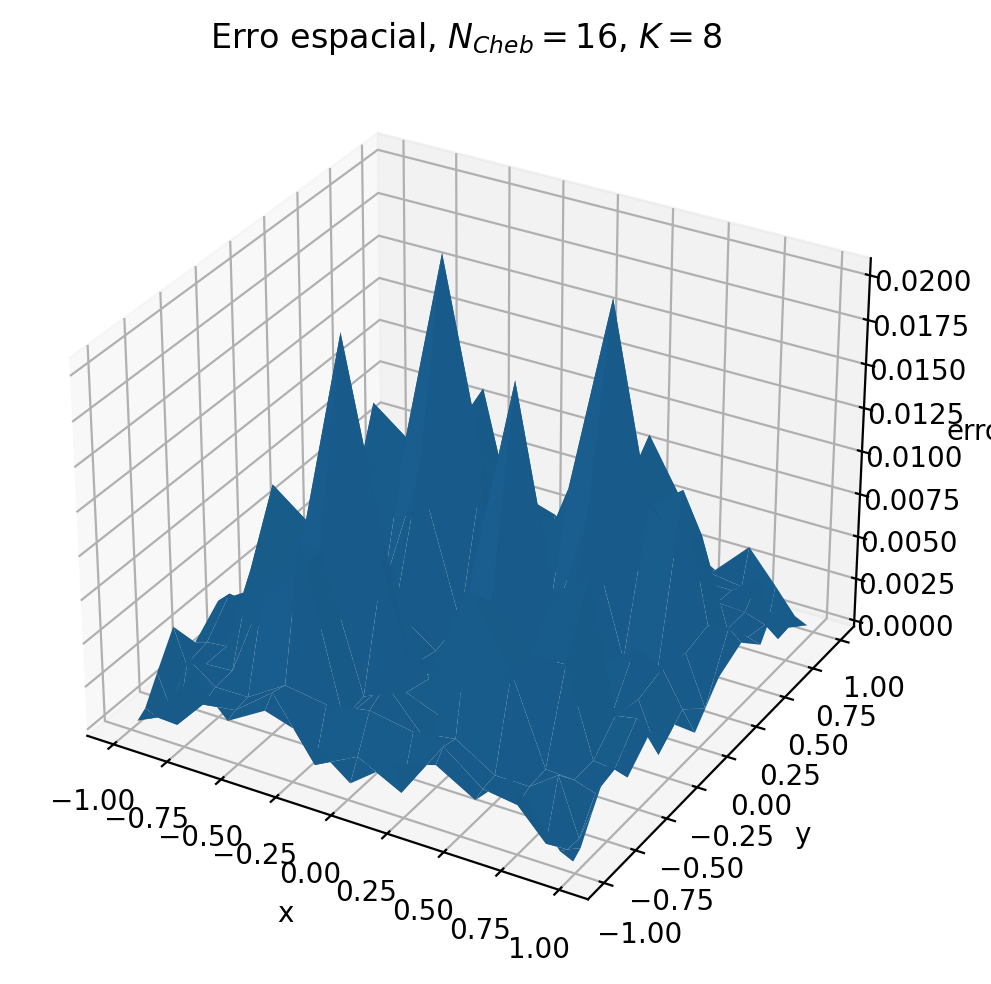
\includegraphics[width=0.72\textwidth]{figuras/superficie_erro_calor2d_N16_K8.png}
\caption{Erro espacial no instante \(t=0\), com \(N_{\text{Cheb}}=16\) e \(K=8\).}
\label{fig:erro_espacial_n16}
\end{figure}

\begin{figure}[h!]
\centering
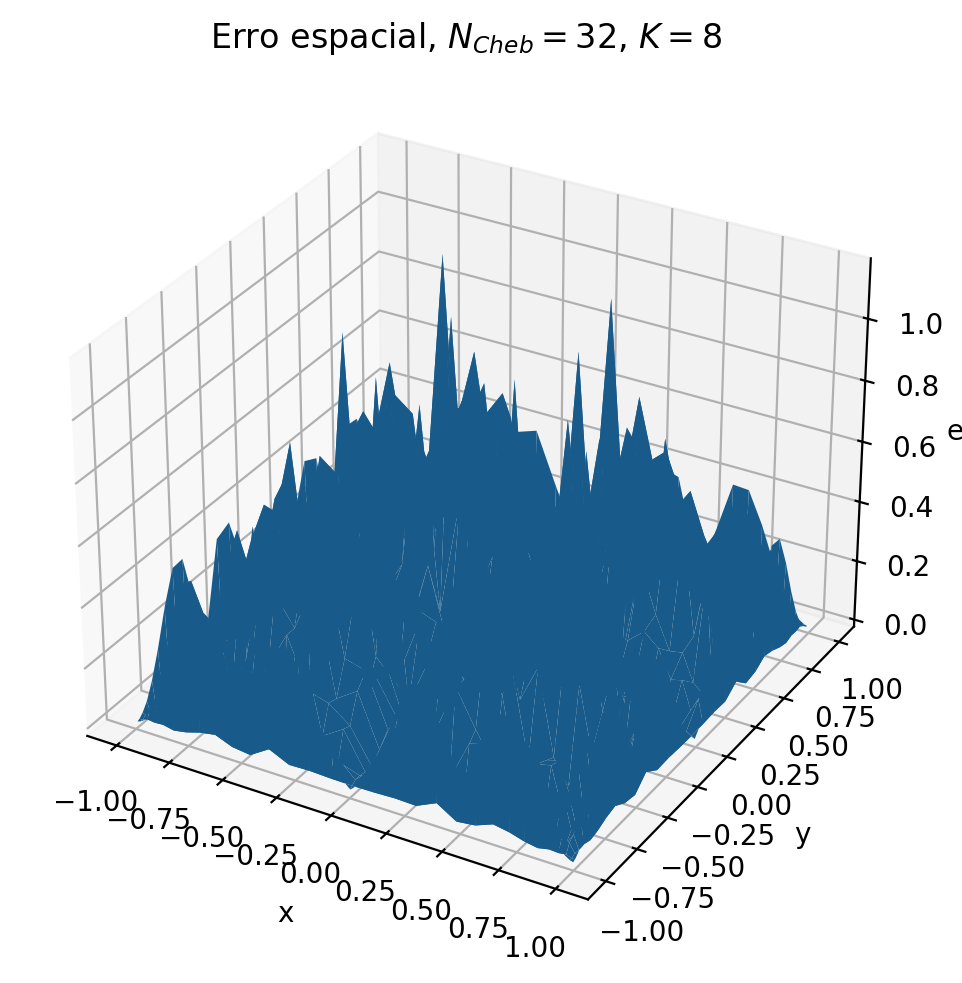
\includegraphics[width=0.72\textwidth]{figuras/superficie_erro_calor2d_N32_K8.png}
\caption{Erro espacial no instante \(t=0\), com \(N_{\text{Cheb}}=32\) e \(K=8\).}
\label{fig:erro_espacial_n32}
\end{figure}

\section{Síntese dos resultados}

Os experimentos numéricos confirmam a coerência da formulação proposta. O teste \(2\times2\) valida a etapa temporal baseada em Fourier, mostrando que poucos modos são suficientes quando a solução possui estrutura harmônica simples. Nesse caso, a solução exata contém apenas os harmônicos \(k=1\) e \(k=2\); por isso, a partir de \(K=2\), a aproximação passa a conter todos os modos relevantes e o erro cai para a ordem da precisão de máquina.

O problema da equação do calor bidimensional evidencia a eficácia da combinação Fourier--Chebyshev. Como a solução fabricada é suave no espaço e periódica no tempo, observa-se o comportamento esperado para métodos espectrais: o erro máximo absoluto decresce rapidamente com o refinamento espacial. Essa queda acentuada está associada ao rápido decaimento dos coeficientes espectrais de funções regulares e à adequação dos pontos de Chebyshev--Gauss--Lobatto para domínios limitados.

Ao mesmo tempo, os resultados mostram uma limitação importante: o ganho de precisão obtido com o aumento de \(N_{\text{Cheb}}\) vem acompanhado do crescimento do número de condição dos sistemas lineares. Esse comportamento é típico de formulações espectrais por colocação, especialmente quando se utilizam matrizes de diferenciação de alta ordem. Assim, os experimentos indicam não apenas a precisão da abordagem espectral, mas também a necessidade de monitorar o condicionamento e os efeitos de arredondamento em discretizações mais refinadas.

Do ponto de vista metodológico, as tabelas fornecem os valores quantitativos principais, enquanto os gráficos ajudam a interpretar a tendência dos experimentos: convergência rápida para soluções suaves, resíduos próximos da precisão de máquina e aumento do condicionamento com o refinamento. Em trabalhos futuros, uma etapa adicional natural será aplicar o mesmo procedimento a forçantes sem solução exata conhecida, usando o resíduo como principal critério de validação, e a problemas não lineares periódicos, nos quais o controle de aliasing por técnicas de \emph{dealiasing} se torna relevante.
